%%%%%%%%%%%%%%%%%%%%%%%%%%%%%%%%%%%%%%%%%%%%%%%%%%%%%%%%%%%%%%%%%%%%%%%%%%
% Copyright (c) 2011, ETH Zurich.
% All rights reserved.
%
% This file is distributed under the terms in the attached LICENSE file.
% If you do not find this file, copies can be found by writing to:
% ETH Zurich D-INFK, Haldeneggsteig 4, CH-8092 Zurich. Attn: Systems Group.
%%%%%%%%%%%%%%%%%%%%%%%%%%%%%%%%%%%%%%%%%%%%%%%%%%%%%%%%%%%%%%%%%%%%%%%%%%

\documentclass[a4paper,twoside]{report} % for a report (default)

\usepackage{bftn} % You need this
\usepackage[pdftex]{graphicx}
\usepackage{color,listings,ctable}

\title{Capability Management in Barrelfish}   % title of report
\author{Akhilesh Singhania, Ihor Kuz}	% author
\tnnumber{013}  % give the number of the tech report
\tnkey{Capability Management} % Short title, will appear in footer

% \date{Month Year} % Not needed - will be taken from version history

\newcommand{\note}[1]{[\textcolor{red}{\textit{#1}}]}

\lstdefinelanguage{Mackerel}{
  morekeywords={datatype,device,register,regtype,constants,type,at,
              many,edit,io,also},
  sensitive=false,
  morecomment=[l]{//},
  morecomment=[s]{/*}{*/},
  morestring=[b]",
  showspaces=false,
  showstringspaces=false,
  showtabs=false,
}

\newcommand{\noarginvocation}[1]{\paragraph{#1 invocation}}
\newcounter{invocArgCnt}
\newenvironment{invocation}[1]{%
  \noarginvocation{#1}
  
  \begin{list}{\emph{Argument~\arabic{invocArgCnt}:}}{%
    \usecounter{invocArgCnt}%
    \setlength{\rightmargin}{\leftmargin}%
    \setlength{\itemsep}{0ex}%
  }
  \renewcommand{\arg}{\item}
}{%
  \end{list}
}

\begin{document}
\maketitle

%
% Include version history first
%
\begin{versionhistory}
\vhEntry{1.0}{08.03.2011}{AS}{Initial version}
\end{versionhistory}

% \intro{Abstract}		% Insert abstract here
% \intro{Acknowledgements}	% Uncomment (if needed) for acknowledgements
% \tableofcontents		% Uncomment (if needed) for final draft
% \listoffigures		% Uncomment (if needed) for final draft
% \listoftables			% Uncomment (if needed) for final draft

\chapter{Introduction}

This document discusses the state of capabilities in the Barrelfish
operating system.

Chapter \ref{chap:known_issues} lists the currently known issues with
capability management and \ref{chap:type_system} discusses the type
system.

Chapter \ref{chap:current_state} discusses the current state of the
implementation in Barrelfish, chapter \ref{chap:db} discusses
different approaches for maintaining a multicore mapping database of
capabilities, chapter \ref{chap:solutions} discusses the requirements
from a correct solution and discusses four different solutions,
chapter \ref{chap:implementation} discusses some Barrelfish specific
challenges in implementing the solutions, and chapter \ref{chap:nyd}
highlights issues not yet covered in this document.

%%%%%%%%%%%%%%%%%%%%%%%%%%%%%%%%%%%%%%%%%%%%%%%%%%%%%%%%%%%%%%%%%%%%%%%%%%%%%%%%
\chapter{Known Issues}\label{chap:known_issues}
\begin{itemize}

\item Kernel operations should not take longer than $O(1)$.  Some
  capability operations are not constant time but can take $O(n)$
  where $n$ is the size of the mapping database. Spending so much time
  in the kernel is detrimental for good scheduling as when in the
  kernel, interrupts are disabled. All non constant time operations
  should be punted to the monitor.

\item When the last copy of a lmp capability or frame capability
  backing ump channels is deleted, should it initiate a connection
  tear down?

\item We have no mechanics for tracking frames mapped into VNodes. So
  that if either is deleted, the entries are properly cleaned up.

\item Multicore capability management. We have an implementation on
  the tip. It is not enabled and has some shortcomings. Not all
  shortcomings are not known however some missing details are
  known. As discussed in chapter~\ref{chap:solutions}, all remote
  relations including descendants, copies, and ancestors must be
  tracked. The implementation only tracks ancestors.

\item Fragmentation of memory. Example: a ram capability of 4GB is
  retyped into two capabilities of 2GB each. One of the 2GB capability
  is deleted. The only way to get a capability to that 2GB back is to
  also delete the other 2GB capability and then retype the 4GB
  capability again.

\item The mapping database is maintained as a doubly linked
  list. Implementing Boolean operations like ``has\_descendants'' and
  ``has\_copies'' require walking the database and testing type
  specific data structures. We feel that these are not efficient or
  robust. If we move the mapping database into the monitor, we think
  that this should at worse become a performance issue and not a
  correctness one.

\item IO space can be treated in a same way as physical memory. So
  instead of using mint operations to update ranges, we use retype
  operations. This is useful as different IO capabilities will have
  the ancestor, descendant, and copy relationships rather than just a
  copy relationship. The former is richer and can offer improved
  maintenance.

\item When a new capability is introduced in a core via cross-core
  send, the kernel must walk the entire mapping database to find the
  appropriate place to insert the capability. The operation is linear
  time. This operation must either happen in the monitor or must be
  made more efficient. If we move the mapping database into the
  monitor, we think that this should at worse become a performance
  issue and not a correctness one.

\item Simon and I had envisioned a memory server mechanism where it
  would delete all ram capabilities after handing them out. This
  allows Simon to implement his version of domain shutdown (discussed
  in a supporting document). In a nutshell, in his system, the spawn
  daemon saves all user dispatcher capabilities and revokes them to
  kill a user dispatcher and repossess its memory. However, there is a
  subtle problem with this mechanism. A malicious dispatcher can
  create loops in its CSpace. E.g. root cnode contains a capability to
  cnode1, cnode1 contains a capability to cnode2, and cnode2 contains
  another capability to cnode1. When a dispatcher does this and the OS
  tries to kill it, root cnode will be deleted and all capabilities
  within it as well. When the OS deletes cnode1, it will check if it
  has copies, which it does so cnode1 will not be deleted. This will
  leak memory in the system.

  To avoid this problem, the OS must maintain ancestors of all
  capabilities that are handed out to user applications and to kill
  the user application, it must revoke the ancestor capabilities.
\end{itemize}

%%%%%%%%%%%%%%%%%%%%%%%%%%%%%%%%%%%%%%%%%%%%%%%%%%%%%%%%%%%%%%%%%%%%%%%%%%%%%%%%
%%%%%%%%%%%%%%%%%%%%%%%%%%%%%%%%%%%%%%%%%%%%%%%%%%%%%%%%%%%%%%%%%%%%%%%%%%%%%%%%
\chapter{Type system}\label{chap:type_system}

In this chapter, we cover the type model of capabilities and the
supported types in Barrelfish.

%%%%%%%%%%%%%%%%%%%%%%%%%%%%%%%%%%%%%%%%%%%%%%%%%%%%%%%%%%%%%%%%%%%%%%%%%%%%%%%%
\section{Type Model}
\note{We do not implement capability rights yet.}
    
\begin{description}
\item[Name] Each type has a unique name.

\item[Origin] A capability type is either \emph{primitive}, which
  means that capabilities of the type may be created only through a
  special process (eg. at boot time), or \emph{derived}, which means
  that capabilities of the type may be created by retyping an existing
  capability. For primitive types, we specify how the capabilities of
  that type are created; for derived types, we specify which
  capability types may be retyped to yield a capability of the given
  type.

\item[Retypability] Some types of capability may be \emph{retyped} to
  create one or more new capabilities of the same or different
  type. If this is the case, we specify for each type from what other types of
  capability it may be retyped.

\item[Mint parameters] It is possible to specify type-specific
  parameters when \emph{minting} capabilities. We specify for each
  type the interpretation of the type-specific parameters. When not
  specified, they are ignored.

\item[Interpretation of rights] The interpretation of the primitive
  capability rights is type-specific. A capability type defines the
  interpretation of these rights, usually in the specification of the
  legal invocations.

\item[Transferability to another core] Depending on its type, it may
  or may not be possible to transfer a capability to another core.

\item[Last copy deleted] The type specific operations to perform when
  the last copy of a capability is deleted. For capability types
    that refer to actual memory, if the last reference to a piece of
    memory is deleted, then the memory must be garbage collected.

\item[Concrete representations] Each capability type has one or more
  representations: in the memory of each core on which it may appear,
  and in a canonical serialised representation used for transferring
  it in a message between cores. These are specified as
  Hamlet\cite{dagand:fof:plos09} data types.

\item[Invocations] Most capability types support one or more
  type-specific operations through the use of the invoke system call.
  (documented in \ref{sec:sys_invoke}).
\end{description}

%%%%%%%%%%%%%%%%%%%%%%%%%%%%%%%%%%%%%%%%%%%%%%%%%%%%%%%%%%%%%%%%%%%%%%%%%%%%%%%%
\section{Types}
  
\subsection{CNode}\label{sec:cnode}

A CNode refers to an array of capabilities of some power-of-two size.
CNodes are used to hierarchically construct the CSpace of a domain, as
described in \ref{sec:cspace}.  All capability management is
performed through invocations on CNodes.

A CNode capability stores a \emph{guard} and \emph{guard size}, which
is expressed as a number of bits. As in guarded page
tables\cite{Liedtke_GPT}, the guard allows the depth of the CSpace
tree to be reduced by skipping levels that would only contain a single
mapping. When resolving a CSpace address that has led to a CNode
capability, the guard is compared with the corresponding number of
bits from the remaining part of the address, and if it does not match,
the lookup fails.

Many CNode invocations require that the caller provide both a CSpace
address and the number of \emph{valid bits} in the address. This
allows the invocations to refer to another CNode capability that is
located at an intermediate level in the tree, and thus would usually
be recursed through by the address resolution algorithm. If the number
of valid bits associated with a CSpace is less than the size of a full
CSpace address, only the least significant bits that are valid, but
starting with the most significant bit thereof, are used, and the
address lookup terminates early.

\begin{description}
\item[Origin] Retyping from RAM type capabilities

\item[Retypability] No

\item[Mint parameters] The mint parameters can be used to set a guard
  on a CNode.
  \begin{itemize}
  \item Parameter 1: The guard to set.
  \item Parameter 2: The size of the guard in bits.
  \end{itemize}

\item[Interpretation of rights] \note{Explain rights and rights mask.
  Capability rights and rights masks are currently not implemented.
  This means that every user domain holding a capability has full
  rights to it.}

\item[Transferability to another core] Yes.  When transfered to
  another core, capability is implicitly retyped to a Foreign CNode
  type. \note{We do not allow CNode type caps to be transferred yet.}

\item[Last copy deleted] When the last copy is deleted, all
  capabilities stored within it are also deleted.

\item[Concrete representations] The in-memory representation of on
  x86-64 is as follows:
    
  \begin{lstlisting}[language=Mackerel]
    datatype cnode_cap "CNode capability" {
      cnode 64 "Physical base address of CNode";
      bits 8 "Number of bits this CNode resolves";
      rightsmask 8 "Capability rights mask";
      guard_size 8 "Number of bits in guard word";
      guard 32 "Bitmask already resolved when reaching this CNode";
    };
    \end{lstlisting}
\end{description}

\begin{invocation}{Mint}\label{sec:mint}
  \arg CSpace address of destination CNode
  \arg Slot number in destination CNode
  \arg CSpace address of source capability
  \arg Number of valid bits in destination CNode address
  \arg Number of valid bits in source capability address
  \arg Type-specific parameter 1
  \arg Type-specific parameter 2
\end{invocation}
The Mint invocation creates a new capability in an existing CNode
slot, given an existing capability.  The new capability will be a copy
of the existing capability, except for changes to the
\emph{type-specific parameters}.

The use of the two type-specific parameters is described along with
the description of the relevant type.

If the destination capability is of type VNode, then instead of a
mint, a page table entry is made into the page table pointed to by the
VNode.  In this case, the source capabilities must be of type VNode,
Frame, or Device Frame.  The first parameter specifies architecture
specific page (table) attributes and the second parameter specifies an
offset from the source frame/device frame to map.
  
\begin{invocation}{Copy}
  \arg CSpace address of destination CNode
  \arg Slot number in destination CNode
  \arg CSpace address of source capability
  \arg Number of valid bits in destination CNode address
  \arg Number of valid bits in source capability address
\end{invocation}
This invocation is similar to Mint, but does not change any
type-specific data.

If the destination capability is of type VNode, then instead of a
copy, a page table entry is made into the page table pointed to by the
VNode.  In this case, the source capabilities must be of type VNode,
Frame, or Device Frame.

\begin{invocation}{Retype}
  \arg CSpace address of source capability to retype
  \arg Type of new objects to create
  \arg Size in bits of each object, for variable-sized objects
  \arg CSpace address of destination CNode
  \arg Slot number in desination CNode of the first created capability
  \arg Number of valid bits in destination CNode address
\end{invocation}

This invocation creates one or more new descendant capabilities of the
specified type in the specified slots, given a source capability and a
destination type.  It will fail if the source or destination are
invalid, or if the capability already has descendants. (some
capability types, currently only the dispatcher type can be retyped
even if it already has descendants).  The destination slots must all
occupy the same CNode.  The permissible source/destination pairs are
shown in \ref{fig:cap_types} and \ref{tab:retype_types}.  The number
of new capabilities created is determined by the size of the source
capability divided by the size of the newly-created objects.

\ctable[
  caption=Permissible types for the Retype invocation,
  label=tab:retype_types,
]{lll}{}{
  \FL Source & Destination & Variable size?\ML
  Physical address range & Physical address range & Yes\NN
  Physical address range & RAM & Yes\NN
  Physical address range & Device frame & Yes\NN
  RAM & RAM & Yes\NN
  RAM & CNode & Yes\NN
  RAM & VNode & No\NN
  RAM & Dispatcher & No\NN
  RAM & Frame & Yes\NN
  Dispatcher & IDC endpoint & No\NN
}

\begin{figure}
  \centering
  \includegraphics[width=.7\columnwidth]{cap_types}
  \caption{Valid capability retyping paths}\label{fig:cap_types}
\end{figure}
  
\begin{invocation}{Delete}
  \arg CSpace address of capability to delete
  \arg Number of valid bits in capability address
\end{invocation}
This invocation deletes the capability at the given address, freeing
the associated CNode slot.

\begin{invocation}{Revoke}
  \arg CSpace address of capability to Revoke
  \arg Number of valid bits in capability address
\end{invocation}
This invocation revokes the capability at the given address.

The capability itself is left untouched while all its descendants and
copies are deleted.

\subsection{Foreign CNode}
\note{This has not been implemented yet}

The foreign CNode capability gives a domain on a core the ability to
specify a capability that actually resides on another core.  This
capability allows for the holder to create local copies of the
capabilities stored in the actual CNode modulo rights as can be
implemented.  The capability tracks on which core the actual CNode
resides.  \note{Full implementation and discussion pending}

\begin{description}
\item[Origin] When a CNode capability are copied to another core.

\item[Retyability] No

\item[Mint parameters] None
  
\item[Interpretation of rights] \note{Explain rights}
  
\item[Transferability to another core] Yes

\item[Last copy deleted] \note{NYI}
  
\item[Concrete representations] The in-memory representation on x86-64 is as follows:
  
  \begin{lstlisting}[language=Mackerel]
    datatype fcnode_cap "Foreign CNode capability" {
      cnode      64  "Physical base address of CNode";
      bits        8  "Number of bits this CNode resolves";
      rightsmask  8  "Capability rights mask";
      core_id     8  "Core id of the core the actual CNode capability
                      resides in";
      guard_size  8  "Number of bits in guard word";
      guard      32  "Bitmask already resolved when reaching this CNode";
    };
  \end{lstlisting}
\end{description}

\note{Discussion pending on invocations}

\subsection{Physical address range}

Most domains will generally not handle capabilities of this type.
They are introduced because the kernel relies on the user-space
software to decide the location of RAM.

By retyping physical address range capabilities to RAM, the caller
guarantees that the underlying region does contain RAM that can safely
be used for storage of kernel objects.  Any domain with access to
physical address range capabilities is therefore a critical part of
the trusted computing base.

\begin{description}
\item[Origin] Created at boot time in the bsp core based on the
  multiboot info.

\item[Mint parameters] None
  
\item[Retyability] To Physical address range, RAM or DevFrame type.
  
\item[Interpretation of rights] \note{Explain rights}
  
\item[Transferability to another core] Yes

\item[Last copy deleted] \note{NYI, maybe inform some special
  dispatcher like memory server}
  
\item[Concrete representations] The in-memory representation on x86-64 is as follows:
  
  \begin{lstlisting}[language=Mackerel]
    datatype physaddr_cap "Physical address range capability" {
      base       64  "Physical base address of region";
      bits        8  "Size of region";
    };
  \end{lstlisting}
\end{description}

\subsection{RAM}

A RAM capability refers to a naturally-aligned power-of-two-sized
region of kernel-accessible memory.

\begin{description}
\item[Origin] Retyping from physical address range capabilities.
  
\item[Retyability] To RAM, Frame, CNode, VNode, or Dispatcher types.
  
\item[Mint parameters] None
  
\item[Interpretation of rights] \note{Explain rights}
  
\item[Transferability to another core] Yes

\item[Last copy deleted] \note{NYI, maybe inform some special
  dispatcher like memory server}
  
\item[Concrete representations] The in-memory representation on x86-64 is as follows:
  
  \begin{lstlisting}[language=Mackerel]
    datatype ram_cap "RAM capability" {
      base       64  "Physical base address of region";
      bits        8  "Size fo region";
    };
  \end{lstlisting}
\end{description}

\subsection{Dispatcher}
This capability type refers to the kernel object associated with a
user-level dispatcher.

\begin{description}
\item[Origin] Retyping from RAM capabilities.
  
\item[Retyability] To IDC Endpoint type
  
\item[Mint parameters] None
  
\item[Interpretation of rights] \note{Explain rights}
  
\item[Transferability to another core] No

\item[Last copy deleted] \note{NYI, maybe inform some special
  dispatcher like spawn daemon}
  
\item[Concrete representations] The in-memory representation on x86-64
  is as follows:
  
  \begin{lstlisting}[language=Mackerel]
    datatype dcb_cap "Dispatcher capability" {
      dcb        64  "Pointer to the in kernel representation of
                      the dispatcher control block";
    };
  \end{lstlisting}
\end{description}

\begin{invocation}{Setup}
  \arg CSpace address of domain's root CNode (root of CSpace)
  \arg Number of valid bits in root CNode address
  \arg CSpace address of domain's root VNode (root page table)
  \arg Number of valid bits in root VNode address
  \arg CSpace address of dispatcher frame (user-level dispatcher
  data) capability
  \arg Whether to make dispatcher runnable
\end{invocation}
This invocation sets any of the above parameters on a dispatcher
object.  If any of the CSpace addresses are null, they are ignored.
Additionally, once all of the parameters are set (either in a single
invocation, or after multiple invocations), and if the runnable flag
is set, the dispatcher is made runnable.  \note{There are additional
  invocations in the code that we have not discussed yet.}

\subsection{IDC Endpoint}
    
Every IDC endpoint refers both to a dispatcher and an \emph{endpoint
  buffer} within that dispatcher. The endpoint buffer is specified as
an offset from the start of the dispatcher frame, and is the location
where the kernel delivers IDC messages. It is also delivered to the
user with an LRPC message.  The initial endpoint offset of an IDC
endpoint capability when it is retyped from a dispatcher capability is
zero; the capability cannot be used to send IDC until the the offset
is specified changed by minting an endpoint to another endpoint.

\begin{description}
\item[Origin] Retyping Dispatcher type capabilities.

\item[Mint parameters] The mint parameters can be used to change the
  badge on the capability
  \begin{itemize}
  \item Parameter 1: The endpoint offset to set on the capability.
  \end{itemize}
  
\item[Retyability] No
  
\item[Interpretation of rights] \note{Explain rights}
  
\item[Transferability to another core] No

\item[Last copy deleted] \note{NYI, inform some entity to initiate
  connection teardown}
  
\item[Concrete representations] The in-memory representation on x86-64
  is as follows:
  
  \begin{lstlisting}[language=Mackerel]
    datatype idc_cap "IDC endpoint capability" {
      listener     64  "Pointer to the in kernel representation of the
                        receiver's dispatcher control block";
      epoffset     64  "Offset of endpoint buffer within dispatcher
                        structure";
    };
  \end{lstlisting}
  
\item[Invocation] Any invocation of an endpoint capability causes the
  entire message to be delivered to the dispatcher to which the
  endpoint refers.
  \end{description}

\subsection{VNode}
A VNode capability refers to a hardware page table and is used to
manage a domain's virtual address space.  Frame and device frame
capabilities can be copied or minted into them or deleted from them by
invoking a CNode.  The architecture may impose limitations on the
capabilities that may be copied into a VNode, or may allow extra
attributes to be set when minting.

\begin{description}
\item[Origin] Retyping from RAM type capabilities.

\item[Retyability] No

\item[Mint parameters] None
  
\item[Interpretation of rights] \note{Explain rights}
  
\item[Transferability to another core] \note{Discussion pending}

\item[Last copy deleted] \note{NYI, initiate mechanisms to unmap from
  associated page tables and remove mapped in page tables and frames}
  
\item[Concrete representations] The in-memory representation on x86-64
  is as follows:
  
  \begin{lstlisting}[language=Mackerel]
    datatype vnode_cap "VNode capability" {
      base     64  "Base address of the page table";
    };
  \end{lstlisting}
\end{description}  

\subsection{Frame}
A frame capability refers to a naturally-aligned power-of-two-sized
region of physical memory that may be mapped into a domain's virtual
address space (by copying it to a VNode).  When a frame capability is
created (ie.~retyped from RAM), the kernel zero-fills the frame.
\note{Is this a good idea? Shouldn't we be able to pre-zero frames?
  -AB}

\begin{description}
\item[Origin] Retyping from RAM type capabilities.
  
\item[Retyability] To Frame type
  
\item[Mint parameters] None
  
\item[Interpretation of rights] \note{Explain rights}
  
\item[Transferability to another core] Yes

\item[Last copy deleted] \note{NYI, initiate unmapping from page
  tables.  We may choose for this to happen when the last copy of a
  frame within a dispatcher is deleted rather than the last copy in
  the entire system.}
  
\item[Concrete representations] The in-memory representation on x86-64
  is as follows:
  
  \begin{lstlisting}[language=Mackerel]
    datatype frame_cap "Frame capability" {
      base       64  "Physical base address of untyped region";
      bits        8  "Size of the region";
    };
  \end{lstlisting}
\end{description}  

\noarginvocation{Identify}
This invocation returns the physical address and size (in bits) of the frame.

\subsection{Device frame}
A device frame capability refers to a naturally-aligned
power-of-two-sized region of physical address space that may be mapped
into a domain's virtual address space (by copying it to a VNode).
Unlike frame capabilties, the kernel does not zero-fill device frame
capabilities upon mapping.  As the name implies, device frames are
typically used for access to memory-mapped devices.

\begin{description}
\item[Origin] Retyping Physical address range type capabilities.
  
\item[Retyability] To Device frame type
  
\item[Mint parameters] None
  
\item[Interpretation of rights] \note{Explain rights}
  
\item[Transferability to another core] Yes

\item[Last copy deleted] \note{NYI, initiate unmapping from page
  tables.  We may choose for this to happen when the last copy of a
  frame within a dispatcher is deleted rather than the last copy in
  the entire system.}
  
\item[Concrete representations] The in-memory representation on x86-64 is as follows:
  
  \begin{lstlisting}[language=Mackerel]
    datatype device_cap "Device Frame capability" {
      base       64  "Physical base address of region";
      bits        8  "Size of the region";
    };
  \end{lstlisting}
\end{description}  

\noarginvocation{Identify} This invocation returns the physical
address and size (in bits) of the frame.

\subsection{IO}
IO capability gives the holder the ability to read and write to IO
ports.

\begin{description}
\item[Origin] A single capability created at boot time in the bsp core.
  
\item[Retyability] No
  
\item[Mint parameters] Used to specify the region of io space the capability can access.
  \begin{itemize}
  \item Parameter 1: Start of the region
  \item Parameter 2: End of the region
  \end{itemize}
  
\item[Interpretation of rights] \note{Explain rights}
  
\item[Transferability to another core] Yes

\item[Last copy deleted] \note{NYI}
  
\item[Concrete representations] The in-memory representation on x86-64 is as follows:
  
  \begin{lstlisting}[language=Mackerel]
    datatype io_cap "IO capability" {
      start      16  "Start of the granted IO range";
      end        16  "End of the granted IO range";
    };
  \end{lstlisting}
\end{description}

\begin{invocation}{Outb}
  \arg IO port number
  \arg Output data
\end{invocation}
This invocation writes a byte to the the specified IO port

\begin{invocation}{Outw}
  \arg IO port number
  \arg Output data
\end{invocation}
This invocation writes a two byte word to the the specified IO port

\begin{invocation}{Outd}
  \arg IO port number
  \arg Output data
\end{invocation}
This invocation writes a four byte to the the specified IO port

\begin{invocation}{Inb}
  \arg IO port number
\end{invocation}
This invocation returns a byte read from the specified IO port.

\begin{invocation}{Inw}
  \arg IO port number
\end{invocation}
This invocation returns a 16-bit word read from the specified IO port.

\begin{invocation}{Ind}
  \arg IO port number
\end{invocation}
This invocation returns a 32-bit doubleword read from the specified IO port.

\subsection{IRQ table capability}
The IRQ table capability allows the holder to configure the user-level
handler dispatcher that will be invoked when the kernel receives
device interrupts.

\begin{description}
\item[Origin] Given to the first domain spawned on a core.
  
\item[Retyability] No
  
\item[Mint parameters] None
  
\item[Interpretation of rights] \note{Explain rights}
  
\item[Transferability to another core] No

\item[Last copy deleted] \note{NYI}
  
\item[Concrete representations] This capability type has no
  representation associated with it as it is used to simply give
  permissions to the holders and does not refer to any kernel data
  structure.
  \end{description}

\begin{invocation}{Set}
  \arg IRQ number
  \arg CSpace address of asynchronous endpoint capability
\end{invocation}
This invocation sets the user-level handler endpoint that will receive
a message when the given interrupt occurs.  While a handler is set,
interrupts will be delivered as IDC messages.


\begin{invocation}{Delete}
  \arg IRQ number
\end{invocation}
This invocation clears the handler for the given IRQ.

\subsection{Kernel Capability}
So far, this capability is treated as the magic capability that gives
the holder a backdoor into performing special operations in the
kernel.

\begin{description}
\item[Origin] Given to the first domain spawned on a core.
  
\item[Retyability] No
  
\item[Mint parameters] None
  
\item[Interpretation of rights] \note{Explain rights}
  
\item[Transferability to another core] No

\item[Last copy deleted] \note{NYI}
  
\item[Concrete representations] The in-memory representation on x86-64 is as follows:
  
  \begin{lstlisting}[language=Mackerel]
    datatype kernel_cap "Kernel capability" {
      kernel_id   8  "Id of the Kernel";
    };
  \end{lstlisting}
\end{description}

\begin{invocation}{Spawn core}
  \arg Apic ID of the core to try booting
  \arg CSpace address of the RAM capability to use to relocate the new kernel
  \arg CSpace address of the Dispatcher capability of the first domain to run
  \arg Number of valid bits for the root CNode to associate with the Dispatcher capability
  \arg CSpace address of the root CNode to associate with the Dispatcher capability
  \arg CSpace address of the VNode to associate with the Dispatcher capability
  \arg CSpace address of the dispatcher frame to associate with the Dispatcher capability
\end{invocation}
The invocation requests the kernel to try booting another core.  The
kernel is to be relocated into the given memory region and to run the
the given domain.

\begin{invocation}{Get core ID}
  \arg None
\end{invocation}
The invocation returns the APIC ID of the core.

\begin{invocation}{Identify capability}
  \arg CSpace address of the capability to identify
  \arg Number of valid bits in the capability
  \arg Location of buffer to hold capability representation
\end{invocation}
The invocation stores the kernel's in-memory representation of the
capability into the given buffer.

\begin{invocation}{Identify CNode, get capability}
  \arg In memory representation of a CNode capability
  \arg Slot number of a capability within the CNode capability
  \arg Location of buffer to hold capability representation
\end{invocation}
The invocation stores the kernel's in-memory representation of the
capability located at the given slot in the given CNode into the given
buffer.

\begin{invocation}{Create capability}
  \arg In memory representation of a capability
  \arg CSpace address of the CNode the place the created capability in
  \arg Number of valid bits in the CSpace address of the CNode
  \arg Slot number to place the capability in
\end{invocation}
Creates the given capability in the given slot in the given CNode.

\begin{invocation}{Create capability}
  \arg In memory representation of a capability
  \arg CSpace address of the CNode the place the created capability in
  \arg Number of valid bits in the CSpace address of the CNode
  \arg Slot number to place the capability in
\end{invocation}
Creates the given capability in the given slot in the given CNode.

\note{The other invocations are outdated and will probably change
  when the monitors are discussed}


%%%%%%%%%%%%%%%%%%%%%%%%%%%%%%%%%%%%%%%%%%%%%%%%%%%%%%%%%%%%%%%%%%%%%%%%%%%%%%%%

\chapter{Current State}\label{chap:current_state}

This chapter will cover how capabilities are stored and what happens
on capability invocation.

\section{Storage}
For security reasons, capabilities are stored in kernel-space and
users are given pointers to them. Each capability is stored in two
separate databases:

\begin{itemize}
\item Each dispatcher has an associated capability space that holds
  all the capabilities it has.  The capability space of a dispatcher
  is implemented using the CNode type capability. Each dispatcher is
  associated with a ``root CNode'' that contains all capabilities the
  dispatcher has.
\item Each core has a mapping database that holds all the capabilities on the
	core. The mapping database is implemented using a tree of the capabilities.
	As discussed later in the chapter, the mapping database stores the
	capabilities in a particular order to facilitate different capability
	operations.
\end{itemize}

\section{Capability invocation}
When a dispatcher invokes a capability, it passes the kernel an
address of the capability in the CSpace it wishes to invoke. The
kernel locates the capability starting from the dispatcher's root
CNode (walks the capability space), verifies that the requested
operation can indeed be performed on the specified capability and then
performs the operation.

\section{Data structures}
Capabilities in Barrelfish are represented by the following data
structures:

{\scriptsize
\begin{verbatim}
    struct mdbnode {
      struct cte *left, *right;  // Links to the mapping database
	  ...
    };

    struct CNode {
      paddr_t cnode;      // Base address of CNode
      uint8_t bits;       // Size in number of bits
      ...
    };

    union capability_u {  // Union of all types of capabilities
      ...
      struct CNode cnode;
      ...
    };

    struct capability {
      enum objtype type;     // Type of capability
      union capability_u u; // Union of the capability
    };

    struct cte {
      struct capability   cap;     ///< The actual capability
      struct mdbnode      mdbnode; ///< MDB node for the cap
    };
\end{verbatim}
}

A capability, \verb|cte|, consists of the actual capability represented by the
``capability'' structure and an entry in the mapping database represented by
the ``mdbnode'' structure. The capability structure contains the type specific
information and the mdbnode contains pointers for the tree representing the
mapping database.

Capabilities can be looked-up in two ways.
\begin{itemize}
\item All capabilities on a core are stored in a mapping database. It
  is possible to reach any capability on the core by traversing from
  any other capability on the core.

\item Capabilities are also stored in the CNode type capability. The
  area of memory identified by the CNode structure is actually an
  array of capabilities. Starting from the ``root CNode'' of a
  dispatcher, it is only possible to reach any capability the
  dispatcher holds.
\end{itemize}

\section{Terminology}

This section discusses some terminology to facilitate the discussion
of capability management.

\subsection{Copy}

A capability X is a copy of a capability Y if:

\begin{itemize}
\item X was copied from Y
\item or Y was copied from X
\item or X was copied from Z and Z was copied from Y
\end{itemize}

\subsection{Descendants}

A capability X is a descendant of a capability Y if:

\begin{itemize}
\item X was retyped from Y

\item or X is a descendant of Y1 and Y1 is a copy of Y

\item or X is a descendant of Z and Z is a descendant of Y

\item or X is a copy of X1 and X1 is a descendant of Y
\end{itemize}

\subsection{Ancestor}

A is a ancestor of B if B is a descendant of A.

\section{CNode invocations}

Most Capabilities have type specific invocations.  Operations on the
CNode capability modifies the capability space of the system. We
discuss how these operations are implemented for a single core system
here.

\note{Invocations on other capability types will probably also modify
  the capability space but alas we don't know how those will work yet.}

\subsection{Retype}

Retyping a capability creates one or more descendants of the
capability. This operation will fail if the capability already has
descendants. The descendants are inserted into a CNode specified by
the operation and into the mapping database right after the retyped
capability.

When a dispatcher issues the retype invocation, the kernel must traverse the
mapping database to ensure that the capability has no descendants, create the
descendants capabilities, insert them in the specified CNode and in the mapping
database.

\subsection{Copy}

Copying a capability creates a new copy of it. The kernel walks the capability
space to find the capability to be copied, creates the copy, and inserts it
into the specified CNode and mapping database.

\subsection{Delete}

Delete removes the specified capability from the CNode in which it
resides and from the mapping database. This operation cannot fail.

The kernel first walks the capability space to locate the capability
to delete. It then walks the mapping database to check if there still
exist copies of the deleted capability. If no copies are found, then
it performs certain operations based on the capability type.

\subsection{Revoke}

Revoking a capability calls delete on all copies and descendants of
it. When the operation returns, the capability will not have any
copies or descendants.

The kernel walks the capability space to find the specified
capability, uses the mapping database to find all copies and
descendants of the specified capability and deletes them.

\subsection{Looking up local copies and descendants}

Due to the capability ordering used by the mapping database, copies are located
adjacant to a capabality and descendants immediately thereafter. Therefore, it
is easy to look up all related copies of a capability on the same core. This
facilitates revocation by looking up all copies and descendants, retypes by
checking for existing descendants, and deltes by checking for copies.

The following pseudo-code looks up all descendants and copies of a
capability given the existence of type specific is\_copy and
is\_descendant functions.

{\scriptsize
\begin{verbatim}
  // Traverse forward
  mdbnode *walk = successor(cap);
  while (walk) {
    // Check if descendant
    if (is_descendant(cap, walk)) {
      // Found a descendant
      goto increment;
    }

    // Check if copy
    if (is_copy(cap, walk)) {
      // Found a copy
      goto increment;
    }

    // Cap is not a descendant or copy
    break;

  increment:
    walk = successor(walk);
  }

  // Traverse backwards
  mdbnode *walk = predecessor(cap);
  while (walk) {
    // Predecessors cannot be descendants

    // Check if copy
    if (is_copy(cap, walk)) {
      // Found a copy
      goto increment;
    }

    // Cap is not a copy
    break;

  increment:
    walk = predecessor(walk);
  }
}
\end{verbatim}
}

\section{Multicore extensions}

The model above only works for a single core system. We have already
extended it to work on multiple cores. Here we discuss these
extensions.

\subsection{Cross-core transfer}

This is a special operation available only to the monitors. This sends
a capability from one core to another.

\subsection{Missing operations}

When a capability is sent to another core, no state is maintained
about it. When checking for capability relations in capability
operations, only the current core is checked. Therefore these
operations are not implemented correctly right now.

\section{Summary}

In this chapter, we presented a background and the current state of
capabilities management in Barrelfish. We can now discuss different
designs for multicore capability management.


%%%%%%%%%%%%%%%%%%%%%%%%%%%%%%%%%%%%%%%%%%%%%%%%%%%%%%%%%%%%%%%%%%%%%%%%%%%%%%%%

\chapter{Maintaining the database}\label{chap:db}
We consider the following approaches for managing the mapping
database.

\note{Use diagrams to better illustrate the discussion below.}

\begin{itemize}
\item \textbf{No partition:} The mapping database and capability space
  for all cores is maintained on a single centralized
  coordinator. Accessing either the capability space or the mapping
  database on any core requires communication with the coordinator.

\item \textbf{Partitioned data structure:} The mapping database for
  all cores is maintained on a single centralized coordinator and the
  capability space is maintained on the local cores. This implies that
  the cte structure is split between the coordinator and the local
  cores. Cores can access the capability space locally and have to
  message the coordinator to access the mapping database. Note that
  split ``capability'' and ``mdbnode'' structures need to maintain
  references to each other.

\item \textbf{Centrally replicated space:} The mapping database and
  the capability space is replicated between a single coordinator and
  the local cores. This implies that two copies of each ``cte''
  structure exist in the system, one on the local core and one on the
  coordinator. Both local core and the coordinator can access the
  mapping database and the capability space.

\item \textbf{Partitioned space:} The mapping database and the
  capability space are maintained on the local cores. The entire
  ``cte'' structure can be accessed locally but capability operations
  will require coordination and communication with remote cores.

\item \textbf{Minimal replication:} The database is partitioned
  between local cores as in the above approach and additionally for
  each capability the cores maintain a cache of its remote relations.
  This is discussed in more detail in section \ref{sec:cache}.
\end{itemize}

We qualitatively compare the above approaches and why the partitioned
space and minimal replication is the best.

\section{Comparison}\label{sec:comparison}
We compare the above approaches in this section.

\subsection{Efficiency of capability invocations}
When a dispatcher invokes a capability, the kernel has to look it up
in the capability space starting from the dispatcher's ``root'' CNode.
If the capability space is not local, then the core has to message the
coordinator to perform the look up. A round trip with the coordinator
is more expensive than a local look up and can become a scalability
bottleneck if we use a single coordinator.

The no partition approach does not maintain a local capability space
and therefore may suffer from poor performance. All other approaches
maintain the capability space locally.

\subsection{Local operations}
Approaches that enable more pure local operations will perform better
as they will reduce the amount of cross-core communication. In the no
partition, partitioned data structure, and replicated space
approaches, no operation can be performed locally. In the partitioned
and minimal replication approaches, certain operations such as copying
capabilities is purely local.

\begin{table*}
\begin{center}
\begin{tabular}{|c|c|c|c|c|c|}
  \hline

  & Cap invocation & Local operations \\
  \hline

  No partition                & - & -   \\ \hline
  Partitioned data structure  & + & -   \\ \hline
  Centrally replicated space  & + & -   \\ \hline
  Partitioned space           & + & +   \\ \hline
  Minimal replication         & + & +   \\ \hline

\end{tabular}
\end{center}
\caption{\label{t:summary}Summary of the different approaches.}
\end{table*}

\subsection{Discussion}
Table \ref{t:summary} summarizes our comparison of the five
approaches. A (+) indicates that the approach performs relatively well
on the given metric and a (-) indicates that the approach performs
relatively poorly. Based on the results, we choose to implement the
partitioned space and minimal replication approaches.

\section{Caching}\label{sec:cache}
The minimal replication approach is characterized as the partitioned
approach with caching the state of remote relations. Capabilities
without remote relations are marked as such and when performing
operations on these no remote communication is required.

When tracking remote relations, three types of relations must be
tracked: copies, descendants, and ancestors. Tracking of remote copies
and descendants is required so that revoke, retype, and delete
operations can be correctly implemented. And capabilities must track
their remote ancestors so if they are deleted, the remote ancestors
can be informed to update the state about their remote descendants.

\subsection{How to maintain the cache?}

\note{Once I discuss total order broadcast with caching, this
  discussion will be revamped.}

There are two ways of maintaining the cache:
\begin{itemize}
\item \textbf{Single bit:} A bit each for the three types of remote
  relations is used. The bits merely indicate the presence of remote
  relations but provide no further information such as which cores
  have the remote relations.

\item \textbf{List:} A list each for the three types of remote
  relations is used. The list contains exact information about which
  cores the remote relations exist on. Uhlig et al [?]'s core mask
  technique can be used to maintain the lists with fixed space
  requirement.
\end{itemize}

\subsubsection{Comparison}
\textbf{Informing existing relations:} When a capability that already
has remote relations is sent to another core, with the single-bit
approach, none of the existing cores with relations have to be
informed, but with the list approach, cores with existing relations
must be informed so they can update their lists.

With both approaches when the last local copy of a capability is
deleted, its remote relations should be informed. This is required in
the list approach so that the cores can update their list and is
required in the single-bit approach so that the cores can determine if
the last remote relation has been deleted and it can mark the
capability as not having the remote relation anymore.

\textbf{Number of cores communicated:} With the single bit approach,
all cores in the system must be contacted, while with the list
approach, just the cores of interest must be contacted.

\textbf{Discussion:} The single-bit approach will probably be more
efficient if the system has few cores and the capabilities that have
remote relations, tend to have them on many cores. The list approach
will have better performance if there are lots of cores in the system
and typically a capability only has relations on a few cores.

\subsection{Where to maintain the cache?}\label{subsec:where}
Imagine that there exists a capability with only local relations. Then
cross-core transfer it applied to it. Should we only mark that
capability as having a remote copy or should we mark all impacted
capabilities accordingly? This section will discuss and compare these
two approaches.

\subsubsection{Mark all}
When cross-core transfer is applied to a capability, it is marked has
having remote copies and all its local relations are also marked as
having the appropriate remote relations. Its local copies will be
marked as having remote copies, its local descendants will be marked
as having remote ancestors, and its local ancestors will be marked as
having remote descendants.

All capabilities maintain complete state of their remote relations at
all times.

\subsubsection{Mark just individual capability}
When cross-core transfer is applied to a capability, it is marked has
having remote copies and none of its local relations are updated.

Capabilities do not maintain the complete state of their remote
relations. Their local relations must be looked up to build the
complete state of their remote relations.

\subsubsection{Comparison}
Both approaches have their specific strengths and weaknesses discussed
here.

\textbf{Cost of cross-core transferring:} When applying cross-core
transfer to a capability, in the mark all approach, all local
relations must be updated whereas in the mark just individual
capability approach, the local relations do not have to be updated.
However, the cross-core transfer operation needs to send full
information about the state of local relations so that the newly
created remote capability can setup its cache properly. Gathering this
information will require accessing all local relations so the mark all
approach represents a small in the operation that must be performed
anyways.

\textbf{Cost of building state of remote relations:} Any capability
operation that requires information on the current state of remote
relations will have to build the full state of remote relations for
the capability. This is done trivially in the mark all approach as
each capability maintains the full state. In the mark just individual
capability approach, all local relations must be accessed to build the
state.

\textbf{Discussion:} Given that the state of remote relations is
trivially constructed in the mark all approach and the cost of
cross-core transfer is only marginally higher than the bare minimum
cost already required, we conclude that the mark all approach is
superior to the mark just individual capability approach.

\subsection{Summary}\label{subsec:cache:summary}
In summary, we have come up with two approaches for the type of cache:
single-bit and list, and we have concluded that the mark all approach
is superior for maintaining the cache.

Maintaining a cache will require the following adjustment to the
capability operations presented above.

\begin{itemize}
\item When cross-core transfer is applied to a capability, it is
  marked as having remote copies. The operation sends information on
  the state of the capability's local and remote relations.

\item When a capability is created due to the cross-core receive
  operation, it incorporates the information about relations sent with
  the cross-core transfer operation.

\item When a copy of a capability is marked as having remote
  relations, the capability is marked as having the same remote
  relations.

\item When a descendant of a capability is marked as having remote
  relations, the capability is marked also marked as having remote
  relations based on the following rules:
  \begin{itemize}
  \item If the descendant has a remote copy, then capability has a
    remote descendant.
  \item If the descendant has a remote descendant, then capability has
    a remote descendant.
  \item If the descendant has a remote ancestor, then capability
    either has a remote copy or an ancestor depending on the outcome
    from the type-specific is\_descendant function.
  \end{itemize}

\item When an ancestor of a capability is marked as having remote
  relations, the capability is marked also marked as having remote
  relations based on the following rules:
  \begin{itemize}
  \item If the ancestor has a remote copy, then capability has a
    remote ancestors.
  \item If the ancestor has a remote descendant, then capability
    either has a remote copy or a remote descendant depending on the
    outcome from the type-specific is\_descendant function.
  \item If the ancestor has a remote ancestor, then capability
    has remote ancestors.
  \end{itemize}

\item When a capability is retyped:
  \begin{itemize}
  \item Its remote copies are marked as having remote descendants
  \item The descendants are marked as having remote ancestors if the
    capability has remote copies.
  \end{itemize}

\item When a capability is copied, the copy is marked as having the
  same remote relations that the capability has.

\item When the last copy of a capability on the core is deleted, its
  remote copies, descendants, ancestors are informed.
\end{itemize}

We now discuss some implications of maintaining a cache.

\textbf{Drawbacks:} Caching introduces the following drawbacks that
the non-caching approach does not suffer from.

\begin{itemize}
\item The application dispatchers must first try to perform the
  capability operations locally and if that fails, then communicate
  with the monitors. If no caching were used, the application
  dispatchers can always directly communicate with the monitor saving
  one superfluous trip into the kernel.

\item As discussed above, caching requires additional overhead in
  keeping the cache consistent.

\item Caching increases the space requirement for maintaining the
  mapping database.
\end{itemize}

Caching can work if typically few capabilities are shared between
cores and can hurt if many capabilities are shared.

\textbf{Decide dynamically:} It is clear that application scenarios
will actually dictate if caching can help and if it does, which type
of caching helps. To support this, Barrelfish can allow applications
to specify which type of caching is well suited for it or the OS can
gather appropriate metrics on application execution and based on that
dynamically update the type of caching used.  For this, we need to
identify the cross-over point where one approach is preferred over the
other.

%%%%%%%%%%%%%%%%%%%%%%%%%%%%%%%%%%%%%%%%%%%%%%%%%%%%%%%%%%%%%%%%%%%%%%%%%%%%%%%%

\chapter{Solutions}\label{chap:solutions}
In this chapter, we discuss mechanisms for implementing the capability
operations. In section \ref{sec:challenges}, we will first discuss the
challenges in correctly implementing the operations by discussing how
executing multiple related operations in parallel can lead to
conflicts and by discussing how an intuitive solution of using
acknowledgments fails to resolve the conflicts. We then present the
requirements from a correct solution in section \ref{sec:requirements}
and compare four different correct solution in section
\ref{sec:solutions}.

\section{Challenges}\label{sec:challenges}
We first discuss the conflicts that can arise if two or more related
operations execute in parallel and then discuss an intuitive but
incorrect solution of using acknowledgments to resolve the conflicts.

\subsection{Conflicts}\label{subsec:conflicts}
Performing overlapping operations on related capability can lead to
conflicts. This section discusses the different types of conflicts
that can arise.

\textbf{Conflicts between two retypes, deletes, or revokes:} If two
different cores are trying to retype, delete, or revoke related
capabilities, then they can conflict. If two different cores try to
retype two copies of a capability, the correct behavior is for one to
succeed and for one to fail. If two cores try to delete the last two
copies of a capability, the correct behavior is for one to just delete
locally and for the other to perform type-specific operations required
when deleting the last copy of a capability. If two cores try to
revoke the same capability, one should succeed, the other should fail
and the capability it was trying to revoke should also be deleted.

\textbf{Conflict between revoke and cross-core transfer:} If a core is
trying to revoke a capability, a copy or descendant of which another
core is trying to transfer, the revoke operation should only finish
when the in-flight capability is also deleted.

\textbf{Conflict between revoke and retype:} If a core is trying to
revoke a capability, a copy or descendant of which another core is
trying to retype, then the retype should either succeed and the new
capabilities be deleted before revoke finishes or the retype should
fail.

\subsection{Non-conflicts}
This section discusses why it is safe to perform other operations in
parallel.

\textbf{Delete and revoke:} Delete at least deletes one capability and
potentially more. If a revoke for a related capability is issued at
the same time, they will overlap and potentially try to perform
redundant operations but these are safe.

\textbf{Delete and transfer:} Delete will delete one capability and
perform a check for copies. The in-flight capability already has a
copy that can satisfy the requirements of delete. If the capability is
also being deleted, it is the same two deletes overlapping which
indeed is a conflict.

\textbf{Retype and delete:} A delete will not conflict with retypes
because it checks for the existence of copies which a successful
retype cannot possibly create. A retype will not conflict with deletes
because no matter when it performs the check for descendants, it will
either see descendants that are about to be deleted or not see them at
all, either of the outcomes is correct.

\textbf{Retype and transfer:} Retype cannot conflict with transfers
because in order to transfer a capability because the capability being
transferred is a copy of an existing capability which does not change
the existing descendants relationships.

\subsection{Incorrect solution}
Since the essential issue with the relation with cross-core transfer
operation is that in-flight capabilities do not exist anywhere, the
sending core can maintain a list of in-flight capabilities which are
garbage collected when the receiver acknowledges the reception of the
capability. This allows the sending core to include the in-flight
capabilities in the search for copies and descendants. As shown below,
this intuitive solution is actually incorrect.

\begin{figure}[t]
 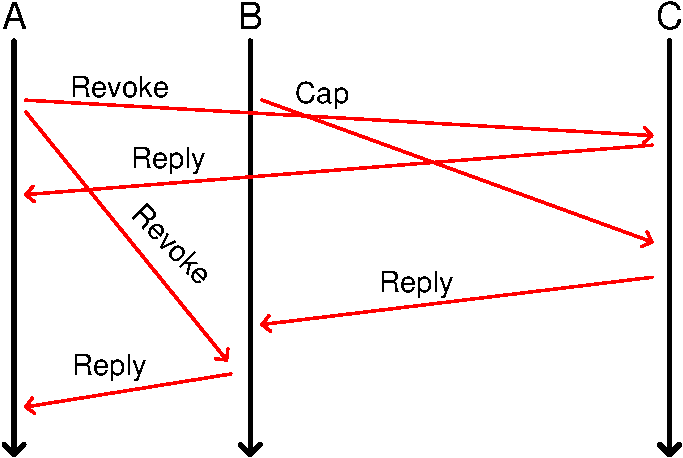
\includegraphics[width=0.75\textwidth]{acks-problem.pdf}
 \caption{Problem with using acknowledments}\label{fig:acks-problem}
\end{figure}

Consider the scenario shown in figure \ref{fig:acks-problem}. The
system consists of three cores \{A, B, C\}, A is trying to revoke a
capability and B is trying to send a copy of the capability to C. A
sends a revoke request to B, C and waits for their acknowledgments. B
sends the capability to C and adds it to its list of in-flight
capabilities. C sees the revoke request first, performs the operation
locally and replies to A. Then it sees the capability sent from B,
inserts it locally and send an acknowledgment to B. B sees the
acknowledgment from C first garbage collecting its list of in-flight
capabilities and then sees the revoke request from A, performs the
revoke locally, and replies to A. A receives replies from both B and C
concluding the revoke operation. The revoke operation has finished and
C still has a copy of the revoked capability.

\section{Requirements from a correct solution}\label{sec:requirements}
A correct solution will enforce the following transactional like and
ordering properties.

\subsection{Transactional properties}
\textbf{Atomic:} If one part of a capability operation fails, then the
entire operation must fail. For example, in a retype operation, the
descendant capabilities can be created in parallel with the check for
existing descendants. If existing descendants are found, then the
newly created descendants must be removed.

\textbf{Consistent:} Every capability operation must leave the system
in a consistent state. For example, if caching is used an operation
deletes the last copy of a capability on a core, then all its remote
relations should be informed and updated before the operation
finishes.

\textbf{Isolation:} The data that has been modified during a
capability operation must not be accessible by other operations till
the operation finishes. For example, if a retype operation has eagerly
created descendants while checking for existing descendants in
parallel, no other capability operation should be able to access the
descendants created eagerly till the retype operation finishes.

\subsection{Ordering}
Section \ref{subsec:conflicts} discusses the two types of conflicts
that can arise when multiple cores try to perform operations on
related capabilities at the time. Correctness can be ensured if the
individual steps (messages) in operations must be executed in some
order.  We provide some background on ordering messages before
discussing the actual ordering requirements.

\textbf{Background on ordering:} Four types of ordering are
possible. We discuss them from the cheapest to the most expensive.

\begin{itemize}
\item No order: Messages can be delivered in any order. This cannot
  happen on Barrelfish.
\item Single Source FIFO (SSF): Messages from the same sender are
  delivered in the order they were sent. This is what currently is
  available on Barrelfish by default.
\item Causal: Messages are delivered based on their partial order
  given by the happens-before relationship. Vector clocks [?] can be
  used to provide causal delivery of messages.
\item Total order: All receivers receive messages in the same
  order. Note that any ordering function can be used to order the
  messages. Further, total order does not imply causal order but if
  the ordering function respects SSF, then total order does imply
  causal order.
\end{itemize}

\subsection{Conflicts with each-other}

\begin{figure}[t]
 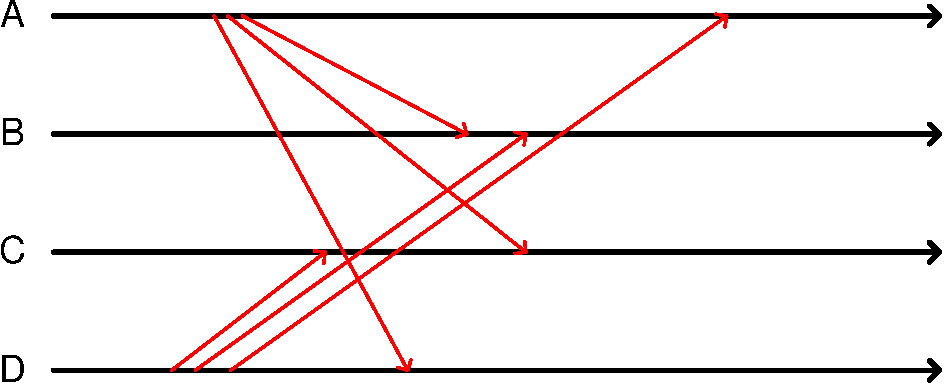
\includegraphics[width=0.75\textwidth]{causal-problem.pdf}
 \caption{Problem with using causal order
   delivery}\label{fig:causal-problem}
\end{figure}

The minimum ordering required for resolving conflicts between retype,
delete, and revoke operations is total order. Figure
\ref{fig:causal-problem} illustrates the reason causal ordering does
not work. Nodes \{A,B,C,D\} each contain copies of the same capability
that \{A,D\} wish to retype at the same time. B receives the message
from A before the message from D, and C receives the D's message
before A's. The messages were delivered in causal order, C will refuse
to A, B will refuse to D not allowing either retype operation to
succeed. Similar examples can be constructed for the delete and revoke
operations as well.

Total order delivery will deliver the messages to B and C in the same
order allowing just one and only one retype to succeed.

\subsection{Conflict between revoke and transfer}
Figure \ref{fig:acks-problem} illustrates the conflict between revoke
and cross-core transfer operation. C sees the message from A before
the message from B. Hence any message it sends to B causally depend
upon the message from A. If this was reflected in the message C sent
to B, then B could delay handling the message till it sees the revoke
request from A. When B receives the revoke request from A, it will
realize that A is trying to revoke an in-flight capability and take
appropriate actions to resolve the issue. The delaying of the message
can be guaranteed by enforcing causal delivery of messages.

\subsection{Conflict between revoke and retype}
The minimum ordering requirement is total. With less stricter
ordering, different cores might see the revoke request and retype
requests in different orders. The retyping core might delete the
source capability but end up creating descendants later.

\section{Solutions}\label{sec:solutions}

We will discuss and compare the following four solutions.

\begin{itemize}
\item Locks
\item Total order broadcast
\item Two phase commit
\item Sequencer
\end{itemize}

\subsection{Locks}\label{subsec:locks}
Locks can be used to enforce the above transactional and ordering
policies. Critical sections can be used to resolve the conflicts
ensuring that \emph{Time-of-check-to-time-of-use} is not violated.

Below, we provide pseudo-code for how capability operations will be
implemented when using a centralized lock and not caching information
about remote relations.

\textbf{Copying a capability:} This operation is safe to be performed
without holding a lock.

\begin{verbatim}
cap_copy(struct cte *cte) {
  create_copies();
}
\end{verbatim}

\textbf{Retyping a capability:} Holding the lock is required to
prevent multiple cores from trying to retype copies of the same
capability. Acquiring the lock is a blocking call during which the
capability might have been deleted so it is important to check that
the capability still exists after the lock is acquired.

\begin{verbatim}
cap_retype(struct cte *cte) {
  errval_t err = success;
  acquire_lock();
  if (cap_exists(cte) == false) {
    err = fail;
    goto done;
  }
  if (has_descendants(cte) == true) {
    err = fail;
    goto done;
  }
  create_descendants(cte);
done:
  release_lock();
  return err;
}
\end{verbatim}

\textbf{Deleting a capability:} If the capability has local copies,
the operation is purely local. Otherwise, holding the lock is required
to ensure that if the last copy of the capability in the system is
being deleted, then the type-specific cleanup operations are executed.

\begin{verbatim}
cap_delete(struct cte *cte) {
  remove_cap(cte);

  if (!requires_typed_ops(cte)) {
    return success;
  }
  if (has_local_copies(cte)) {
    return success;
  }

  errval_t err = success;
  acquire_lock();
  if (!cap_exists(cte) {
    goto done;
  }

  if (!has_copies(cte) {
    type_specific_ops(cte);
  }

done:
  release_lock();
  return err;
}
\end{verbatim}

\textbf{Revoking a capability:} Holding the lock is required to ensure
that if multiple cores are trying to revoke related capabilities, only
one succeeds. This is why the code below ensures that the capability
still exists after acquiring the lock.

\begin{verbatim}
cap_revoke(struct cte *cte) {
  errval_t err = success;
  acquire_lock();
  if (!cap_exists(cte) {
    err = fail;
    goto done;
  }

  while(has_descendants(cte) {
    struct cte *dest = get_next_descendant(cte);
    remove_cap(dest);
  }
  while(has_copies(cte) {
    struct cte *dest = get_next_copy(cte);
    remove_cap(dest);
  }

done:
  release_lock();
  return err;
}
\end{verbatim}

\textbf{Cross-core transferring a capability:} Holding the lock is
required to conflicts between the above capability operations and
cross-core transfer operation. The sender acquires the lock and sends
the capability. The receiver creates the capability and releases the
lock.

\begin{verbatim}
cap_send(struct cte *cte, coreid_t dest) {
  acquire_lock();
  if (cap_exists(cte) == false) {
    return fail;
  }
  send_cap(cte, dest);
}

cap_receive(struct cte *cte) {
  create_cap(cte);
  release_lock();
  return_success_to_app();
}
\end{verbatim}

\subsubsection{Caching remote relations}
If remote relations are cached, then the cache has to be kept
consistent when capability operations change the state of
relations. Below we describe the modifications that will be required
in the above pseudo-code to keep the cache consistent. Note that our
cache can be seen as eager replication. As discussed in section
\ref{subsec:where}, we will be using the mark all approach to maintain
the cache.

\textbf{Copying a capability:} When the new copy is created, its cache
of remote relations is set equal to the cache from the capability it
was copied from.

\textbf{Retyping a capability:} If the capability does not have remote
copies and descendants, the operation is purely local and the lock is
not required. If the operation is not local, then the lock is
acquired, checks for existence of capability and for descendants and
is made, the capability is retyped, and remote relations are updated
based on the rules presented in section \ref{subsec:cache:summary}.

\begin{verbatim}
cap_retype(struct cte *cte) {
  if (has_local_descendants(cte) == true) {
    return fail;
  }

  if (!has_remote_copies(cte) && !has_remote_descendants(cte)) {
    create_descendants(cte);
    return success;
  }

  if (has_remote_descendants(cte)) {
    return fail;
  }

  errval_t err = success;
  acquire_lock();
  if (!cap_exists(cte)) {
    err = fail;
    goto done;
  }

  if (has_remote_descendants(cte)) {
    err = fail;
    goto done;
  }
  if (has_local_descendants(cte)) {
    err = fail;
    goto done;
  }

  create_descendants(cte);
  update_relations(cte);

done:
  release_lock();
  return err;
}
\end{verbatim}

\textbf{Deleting a capability:} If the capability has local copies or
no remote relations, the operation is purely local. Otherwise, the
lock is required and the remote relations must be updated.

\begin{verbatim}
cap_delete(struct cte *cte) {
  remove_cap(cte);

  if (!requires_typed_ops(cte)) {
    return success;
  }
  if (has_local_copies(cte)) {
    return success;
  }

  if (!has_remote_relations(cte)) {
    type_specific_ops(cte);
    return success;
  }

  acquire_lock();
  if (!cap_exists(cte)) {
    goto done;
  }
  if (!has_copies(cte) {
    type_specific_ops(cte);
  }
  update_remote_relations(cte);
  remove_cap(cte);
  release_lock();
done:
  return success;
}
\end{verbatim}

\textbf{Revoking a capability:} If the capability has no remote
relations, the operation is purely local. Otherwise, the lock is
required.

\begin{verbatim}
cap_revoke(struct cte *cte) {
  if (!has_remote_relations(cte)) {
    while(has_descendants(cte) == true) {
      struct cte *dest = get_next_descendant(cte);
      remove_cap(dest);
    }
    while(has_copies(cte) == true) {
      struct cte *dest = get_next_copy(cte);
      remove_cap(dest);
    }
    return success;
  }

  errval_t err = success;
  acquire_lock();
  if (!cap_exists(cte)) {
    err = fail;
    goto done;
  }

  while(has_descendants(cte) == true) {
    struct cte *dest = get_next_descendant(cte);
    remote_cap(dest);
  }
  while(has_copies(cte) == true) {
    struct cte *dest = get_next_copy(cte);
    remote_cap(dest);
  }
  release_lock();
done:
  return err;
}
\end{verbatim}

\textbf{Cross-core transferring a capability:} The remote relations
cache on local and remote capabilities is updated as presented in
section \ref{subsec:cache:summary}.

\subsubsection{Multiple locks}
\note{NYI}
If a single lock for the entire system is used, only one capability
operation can be performed at any given moment limiting the available
potential for parallelism. By using different locks for unrelated
capabilities, multiple capability operations can proceed in
parallel. Using multiple locks will increase the space requirement but
will also improve parallelism.

\note{Multiple locks are not straight-forward. Ancestors reference
  more memory than descendants do.}

\note{Can a copy lock for delete, a descendant lock for retype, and
  both for revoke work?}

\subsection{Total order broadcast}
\note{Use a single data structure for all pending cap operations.}

The required transactional and ordering guarantees can be provided by
ensuring that messages for related capabilities are delivered in the
same order on all cores. Note that causal order delivery resolves the
conflict between retype, delete, revoke and cross-core transfer
operation but not within the retype, delete, revoke operations.

Below we present pseudo-code for how the capability operations will be
implemented when not caching information about remote relations.

\textbf{Copying a capability:} This operation is safe to be performed
without any ordering requirements.

\textbf{Deleting a capability:} If the capability does not require
type-specific operations or has local copies, the operation succeeds.
Or else, local state is created and a message is broadcast to all
cores.

\begin{verbatim}
cap_delete(struct cte *cte) {
  if (!requires_typed_ops(cte) || has_local_copies(cte)) {
    remove_cap(data->cte);
    return success;
  }

  struct delete_data *data = malloc(sizeof(struct delete_data));
  delete_data_initialize(data, cte);
  outstanding_delete_list->add(data);
  send_delete_request_bcast(TOTAL_ORDER, data);
}
\end{verbatim}

If a core receives a delete request broadcast and it was the sender of
the message, it removes the capability and returns. If the core was
not the sender of the message, then it replies with the state of local
copies of the specified capability.

\begin{verbatim}
delete_request_bcast(coreid_t from, struct delete_request *data) {
  if (from == my_core_id) {
    remove_cap(data->cte);
    return;
  }

  send_delete_reply(from, data, has_local_copies(data->cte));
}
\end{verbatim}

Finally, when a core receives a reply from a delete request, if a
remote copy is found, no type-specific cleanup is required and the
operation finishes. If all replies have been aggregated and no copies
were found, then the type-specific cleanups are performed and then the
operation finishes.

\begin{verbatim}
delete_reply(coreid_t from, bool has_copies) {
  struct cte *my_data = outstanding_deletes_list->get(data);
  if (!my_data) {
    return;
  }

  if (has_copies) {
    outstanding_deletes_list->remove(my_data);
    return;
  }

  increment_replies(my_data);
  if (seen_all_replies(my_data)) {
    type_specific_ops(cte);
    outstanding_deletes_list->remove(my_data);
  }
}
\end{verbatim}

Since the deleting cores remove the capability when they receive the
broadcast, when multiple cores are trying to delete copies, the last
core's broadcast will see no copies while other cores will see copies.

\note{Malloc probably means unbounded memory requirement.}

\textbf{Retyping a capability:} If the capability has local
descendants, then the operation fails. Else, a retype request
broadcast is sent.

\begin{verbatim}
cap_retype(struct cte *cte) {
  if (has_local_descendants(cte)) {
    return fail;
  }

  struct retype_data *data = malloc(sizeof(struct retype_data));
  retype_data_initialize(data, cte);
  outstanding_retypes_list->add(data);
  send_retype_request_bcast(data);
}
\end{verbatim}

When a core receives a retype request broadcast and it was the sender
of the message, one of two things may have happened. Either the core
had already received a broadcast from another core trying to retype
the same capability in which case the receiver's operation has failed
and the state for the request has been removed or the core can succeed
in retyping the capability and updates its state accordingly. If the
core was not the sender of the broadcast, it sends a reply to the
sender with the state of its local descendants. Then the core checks
if it has an outstanding retype request for the capability. If it does
and its request has not been delivered yet, its retype fails. An error
is sent to the application and the state is garbage collected.

\begin{verbatim}
retype_request_bcast(coreid_t from, struct retype_request *data) {
  if (from == my_core_id) {
    struct cte *my_data = outstanding_retypes_list->get(data);
    if (!my_data) {
      return;
    }
    my_data->can_succeed_flag = true;
    return;
  }

  send_retype_reply(from, data, has_local_descendants(data->cte));
  struct cte *my_data = outstanding_retypes_list->get(data);
  if (!my_data) {
    return;
  }

  if (!my_data->success_flag) {
    outstanding_retypes_list->remove(my_data);
    return_failure_to_app();
  }
}
\end{verbatim}

When a core receives a reply to the retype request broadcast, the
operation may already have been failed, in which case the reply is
ignored. If the operation has not been canceled yet, then if the reply
indicates no descendants, the operation can still succeed. If all
replies are seen then the retype operation succeeds.

\begin{verbatim}
retype_reply(struct retype_request *data, bool has_descendants) {
  struct cte *my_data = outstanding_retypes_list->get(data);
  if (!my_data) {
    return;
  }

  if (has_descendants) {
    outstanding_retypes_list->remove(my_data);
    return_failure_to_app();
    return;
  }

  increment_replies(my_data);
  if (seen_all_replies(my_data)) {
    create_descendants();
    outstanding_retypes_list->remove(my_data);
    return_success_to_app();
  }
}
\end{verbatim}

This resolves the conflicts between two retypes. The conflict between
retype and revoke are discussed below.

\note{Malloc probably means unbounded memory requirement.}

\textbf{Revoking a capability:} The core initializes some local state
and then broadcasts a revoke request to all cores in the system.

\begin{verbatim}
cap_revoke(struct cte *cte) {
  struct revoke_data *data = malloc(sizeof(struct revoke_data));
  revoke_data_initialize(data, cte);
  outstanding_revokes_list->add(data);
  send_revoke_request_bcast(TOTAL_ORDER, data);
}
\end{verbatim}

When a core receives a revoke request broadcast, if the core was
trying to retype a related capability, then it fails the retype
operation. If it is not trying to revoke the capability itself, it
simply revokes the capability locally and sends a reply. If the core
is trying to revoke the same capability but it was not the sender of
the broadcast, then this core's revoke operation fails.

\begin{verbatim}
revoke_request_bcast(coreid_t from, struct revoke_request *data) {

  if (related_retype_in_progress(data->cte)) {
    outstanding_retypes_list->remove(data);
    return_fail_to_app();
  }

  struct cte *my_data = outstanding_revokes_list->get(data);
  if (!my_data) {
    revoke_locally(data->cte);
    send_revoke_reply(from, data);
    return;
  }

  if (from != my_core_id && !my_data->success_flag) {
    outstanding_revokes_list->remove(my_data);
    send_revoke_reply(from, data);
    return_failure_to_app();
    return;
  }

  my_data->success_flag = true;
}
\end{verbatim}

When a core receives a reply from the broadcast, it aggregates them
till it has heard back from all cores in the system and then sends a
success to the application.

\begin{verbatim}
revoke_reply(struct revoke_request *data) {
  struct cte *my_data = outstanding_revokes_list->get(data);
  if (!my_data) {
    return;
  }

  increment_replies(my_data);
  if (seen_all_replies(my_data) && !my_data->sent_transfer_cap_delete_flag) {
    outstanding_revokes_list->remove(my_data);
    return_success_to_app();
  }
}
\end{verbatim}

\textbf{cross core transfer:} When sending a capability to another
core, the sending core creates local states and broadcasts the send
message to all cores in the system.

\begin{verbatim}
cap_transfer(struct cte *cte, coreid_t to) {
  struct transfer_data *data = malloc(sizeof(struct transfer_data));
  transfer_data_initialize(data, cte);
  outstanding_transfers_list->add(data);
  send_transfer_request_bcast(TOTAL_ORDER, data, to);
}
\end{verbatim}

When a core receives the capability transfer broadcast, it checks
against the state of current capability operations in progress and
takes appropriate actions if they are related.

If a revoke operation is in progress that is trying to revoke a copy
or an ancestor of the capability being transferred, the broadcast will
indicate that the system indeed has more copies and descendant of the
capability being revoked which must be deleted. If the receiver was
also the recipient of the capability, it does not create it and
returns an error to the sender of the capability or else the receiver
sends a message to the core to which the capability is being
transferred to requesting it to delete the capability.

\begin{verbatim}
transfer_request_bcast(coreid_t from, struct transfer_data *data, coreid_t to) {
  struct cte *my_data;
  my_data = outstanding_revokes_list->get(data);
  if (my_data) {
    if (to == my_core_id) {
      send_transfer_reply(from, FAILURE_REVOKED, data);
      return;
    }

    my_data->sent_transfer_cap_delete_flag = true;
    send_delete_transferred_cap_request(to, data);
  }

  if (to != my_core_id) {
    return;
  }

  my_data = pending_delete_for_transferred_cap_list->get(data);
  if (my_data) {
    pending_delete_for_transferred_cap_list->remove(my_data);
    send_delete_transferred_cap_reply(my_data->from);
    send_transfer_reply(from, FAILURE_REVOKED, data);
  }

  cap_create(data->cte);
  send_transfer_reply(from, SUCCESS);
}
\end{verbatim}

When the sender of the capability gets a reply from the receiver, it
forwards the error code to the application and garbage collects its
state.

\begin{verbatim}
transfer_reply(errval_t err, struct transfer_request *data) {
  my_data = outstanding_transfers_list->get(data);
  outstanding_transfers_list->remove(data);
  return_err_to_app(my_data->app, err);
}
\end{verbatim}

If a revoke was in progress during the transfer of the capability, the
core revoking the capability sends a message to the receiver of the
transferred capability to delete it. When the receiver receives this
message, it may or may not have received the capability yet. If it has
already received the capability, it deletes or else it establishes
some state to delete when it is later received.

\begin{verbatim}
delete_transferred_cap_request(coreid_t from, struct data *data) {
  if (cap_exists(data->cte)) {
    remove_cap(cte);
    send_delete_transferred_cap_reply(from);
    return;
  }

  struct pending_delete_for_transferred_cap *my_data =
    malloc(sizeof(struct pending_delete_for_transferred_cap));
  pending_delete_for_transferred_cap_initialize(my_data);
  pending_delete_for_transferred_cap_list->add(my_data);
}
\end{verbatim}

\begin{verbatim}
delete_transferred_cap_reply(struct data *data) {
  my_data = outstanding_revokes_list->get(data);
  if (my_data) {
    return;
  }

  my_data->sent_transfer_cap_delete_flag = false;
  if (seen_all_replies(my_data)) {
    outstanding_revokes_list->remove(my_data);
    return_success_to_app();
  }
}
\end{verbatim}

\note{Caching NYI}

\subsection{Two phase commit}
\note{NYI}
Use 2pc.

\subsection{Sequencer}
\note{NYI}
Use a sequencer. This will order whole operations.

\subsection{Comparison}
Compare the approaches

%%%%%%%%%%%%%%%%%%%%%%%%%%%%%%%%%%%%%%%%%%%%%%%%%%%%%%%%%%%%%%%%%%%%%%%%%%%%%%%%

\chapter{Implementation details}\label{chap:implementation}

\begin{itemize}
\item Using THC
\item Using RPC between app and monitor
\item Using RPC between monitors
\item Everything having ancestors on memserv
\item Optimization: monitor caches root cnodes
\item Bootstrap
\item How to put enum objtype in interface file?
\item Two types of ifdefs: type of caching (none, list, or bits) and
  type of mgmt
\end{itemize}

\section{Performing capability operations}
If caching is not used, then the application knows for which
operations it must contact the monitor and does so directly without
requesting the kernel to try to perform the operation first.

If caching is used, then the application should try to perform the
operation via the kernel first. If the capability does have remote
relations, the kernel returns an appropriate error to the application
in which case it contacts the monitor.

\section{Sharing mdb between kernel and monitor}
When the application wants the monitor to perform an operation for it,
it passes the monitor its root CNode and all the required parameters.

%%%%%%%%%%%%%%%%%%%%%%%%%%%%%%%%%%%%%%%%%%%%%%%%%%%%%%%%%%%%%%%%%%%%%%%%%%%%%%%%

\chapter{Not Yet Discussed}\label{chap:nyd}

Things that I know that I need to discuss.

\begin{itemize}

\item The OS does not guarantee which order the operations will be
  performed in. The user must enforce the ordering herself.

\item Partitioned approach with caching is eager replication. Consider
  lazy replication.
\end{itemize}

\bibliographystyle{plain}
\bibliography{defs,barrelfish}

\end{document}
